\begin{frame}{Задача двух тел}
	\begin{columns}[T] % Выравнивание колонок по верхнему краю
		\small
		\begin{column}{0.625\textwidth}
			\begin{tcolorbox}[
				colframe=DeepBlue!35,       % Тонкий приглушенный синий контур
				colback=DeepBlue!1!Ivory,    % Мягкий фон, плавно сливающийся с Ivory
				boxrule=0.5pt,               % Ультратонкая рамка
				arc=3pt,                     % Легкое скругление
				top=2pt, bottom=2pt, left=4pt, right=4pt,
				before=\vspace{2pt}, after=\vspace{0pt}
				]
				\small
				\vspace{-6pt}
				\[
				\begin{cases}
					u_1'' = -\dfrac{u_1}{r^3}, \; u_1(0) = 1 - e, \; u_1'(0) = 0 \\[10pt]
					u_2'' = -\dfrac{u_2}{r^3}, \; u_2(0) = 0, \; u_2'(0) = \sqrt{\dfrac{1+e}{1-e}}
				\end{cases}
				\]
				\vspace{-4pt}
				\centering {\footnotesize $r = \sqrt{u_1^2 + u_2^2}, \quad t \in [0, T], \quad e \in [0, 1)$}
			\end{tcolorbox}
		\end{column}
		

		\begin{column}{0.375\textwidth}
			\begin{tcolorbox}[
				colframe=DeepBlue!35, 
				colback=DeepBlue!1!Ivory, 
				boxrule=0.5pt, arc=3pt, 
				top=2pt, bottom=2pt, left=4pt, right=4pt,
				before=\vspace{2pt}, after=\vspace{0pt}
				]
				\small
				\vspace{-6pt}
				\[
				\begin{cases}
					u_1(t) = \cos(\theta_E) - e \\[8pt]
					u_2(t) = \sqrt{1 - e^2} \sin(\theta_E)
				\end{cases}
				\]
				\vspace{-2pt}
				\centering {\footnotesize $\theta_E - e \sin(\theta_E) - t = 0$}
			\end{tcolorbox}
		\end{column}
		
	\end{columns}
	\vspace{0.1cm}
	\centering
	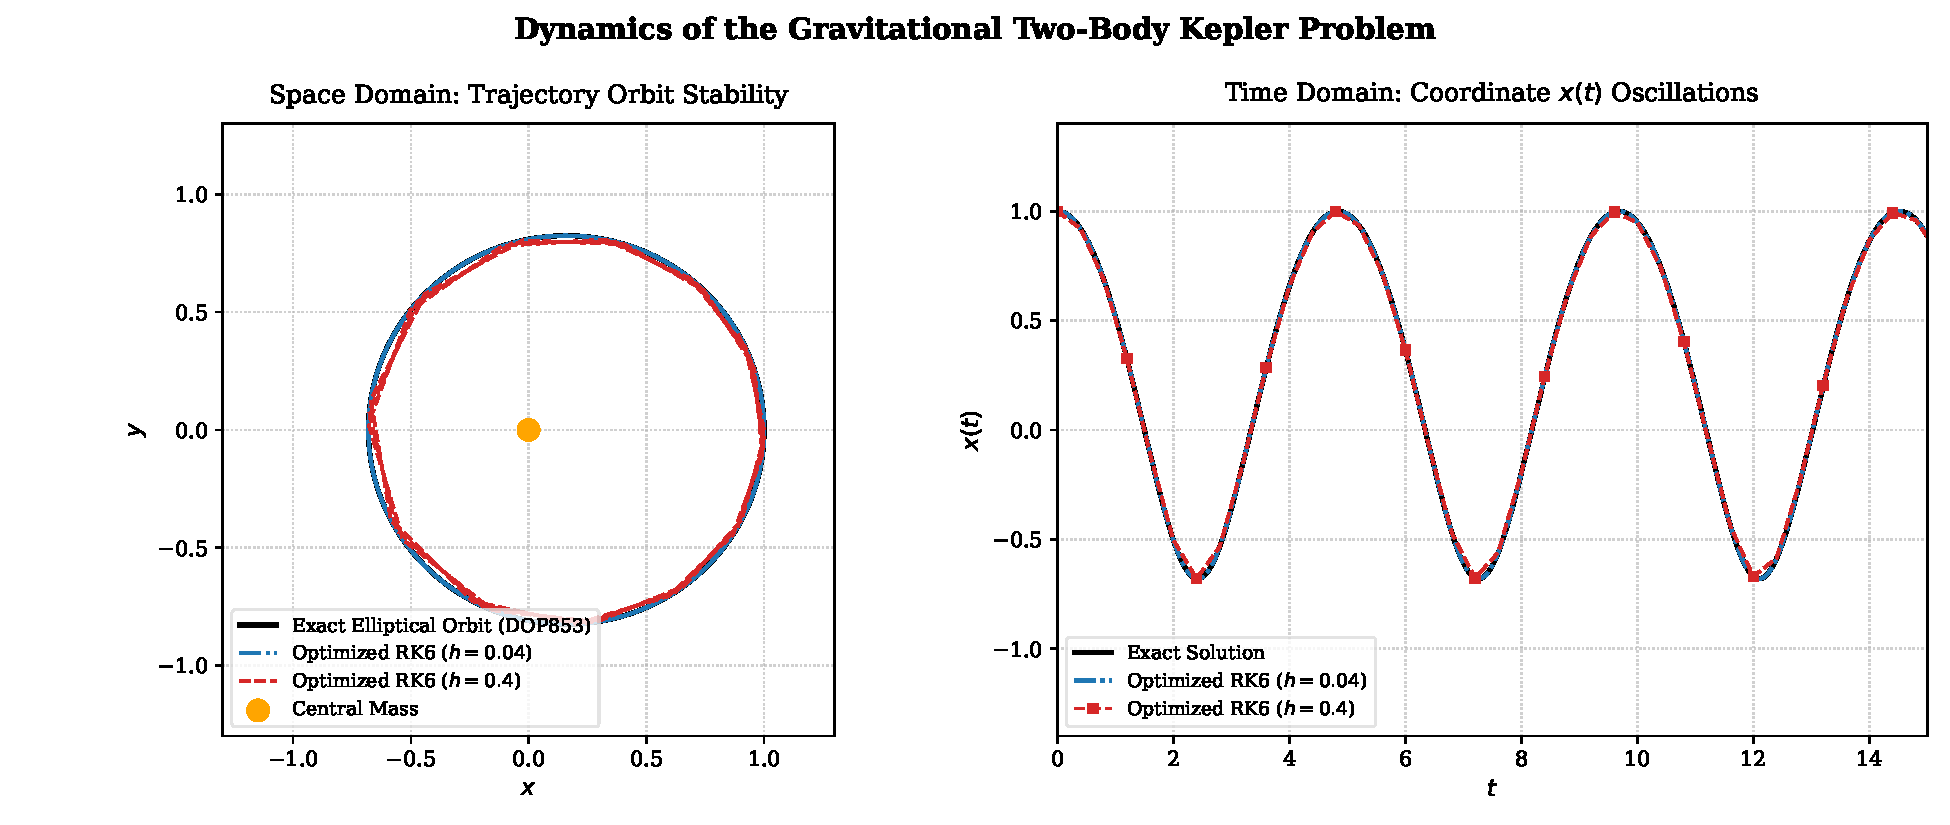
\includegraphics[height=0.495\textheight]{../code/results/visualization/twobody_orbit_comparison}
	
	\begin{tikzpicture}[remember picture, overlay]
		\node[opacity=0.05, inner sep=0pt] at (current page.center) 
		{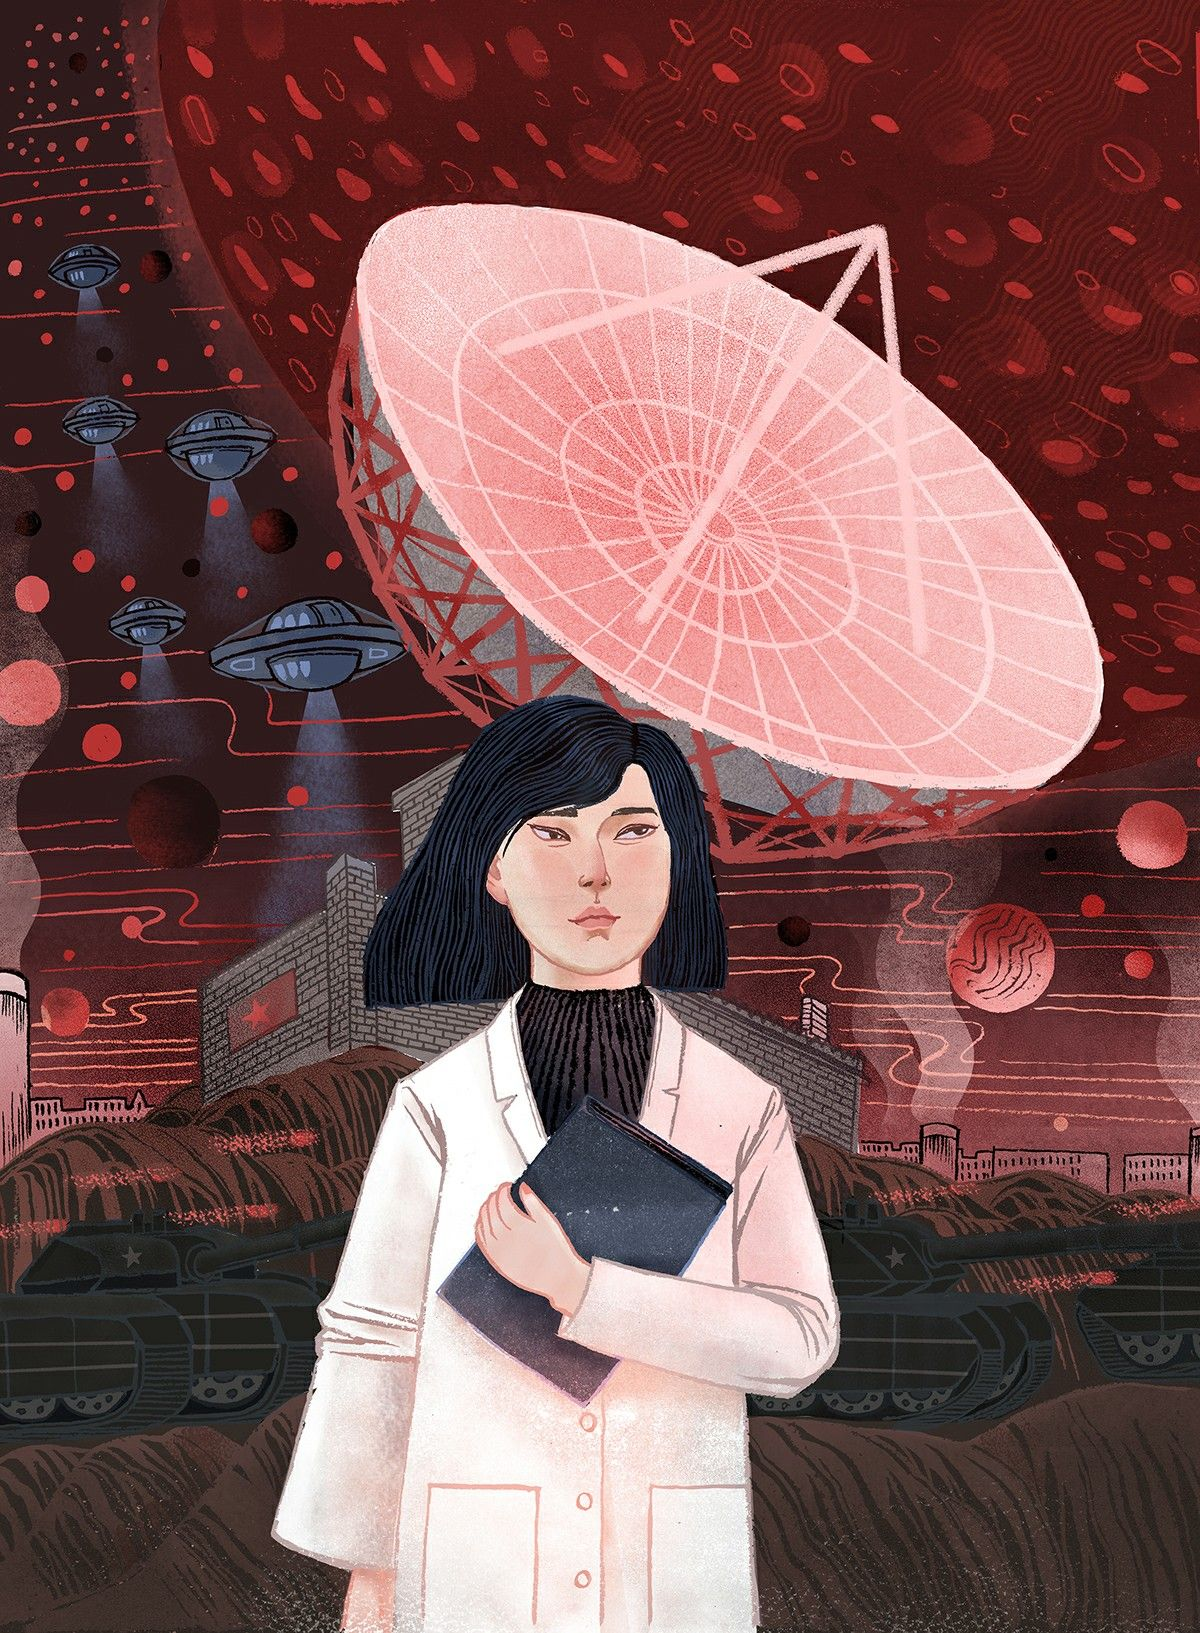
\includegraphics[width=\paperwidth]{three_body}}; 
	\end{tikzpicture}
	
\end{frame}